% ==============================================================================
% Modelo para Especificação de Projeto de Software
% Prof. Vítor E. Silva Souza - NEMO/UFES :: DI/UFES :: PPGI/UFES
%
% Baseado em abtex2-modelo-trabalho-academico.tex, v-1.9.2 laurocesar
% Copyright 2012-2014 by abnTeX2 group at http://abntex2.googlecode.com/ 
%
% This work may be distributed and/or modified under the conditions of the LaTeX 
% Project Public License, either version 1.3 of this license or (at your option) 
% any later version. The latest version of this license is in
% http://www.latex-project.org/lppl.txt.
%
% IMPORTANTE:
% Instruções encontram-se espalhadas pelo documento. Para facilitar sua leitura,
% tais instruções são precedidas por (*) -- utilize a função localizar do seu
% editor para passar por todas elas.
% ==============================================================================

% Usa o estilo abntex2, configurando detalhes de formatação e hifenização.
\documentclass[
	12pt,				
	oneside,		
	a4paper,			
	english,			% Idioma adicional para hifenização.
	french,				% Idioma adicional para hifenização.
	spanish,			% Idioma adicional para hifenização.
	brazil				% O último idioma é o principal do documento.
	]{abntex2}


%%% Importação de pacotes. %%%

% Conserta o erro "No room for a new \count". 
% O comando \reserveinserts deve ser comentado ou não, dependendo da versão do LaTeX.
\usepackage{etex}
%\reserveinserts{28}

% Usa a fonte Latin Modern.
\usepackage{lmodern}

% Seleção de códigos de fonte.
\usepackage[T1]{fontenc}

% Codificação do documento em Unicode.
\usepackage[utf8]{inputenc}

% Usado pela ficha catalográfica.
\usepackage{lastpage}

% Indenta o primeiro parágrafo de cada seção.
\usepackage{indentfirst}

% Controle das cores.
\usepackage[usenames,dvipsnames]{xcolor}

% Inclusão de gráficos.
\usepackage{graphicx}

% Melhor controle de leiaute de tabelas.
\usepackage{tabularx}
\usepackage{colortbl}
\usepackage{longtable}
\usepackage{pdflscape}

% Inclusão de páginas em PDF diretamente no documento (para uso nos apêndices).
\usepackage{pdfpages}

% Para melhorias de justificação.
\usepackage{microtype}

% Citações padrão ABNT.
\usepackage[brazilian,hyperpageref]{backref}
\usepackage[alf]{abntex2cite}	
\renewcommand{\backrefpagesname}{Citado na(s) página(s):~}		% Usado sem a opção hyperpageref de backref.
\renewcommand{\backref}{}										% Texto padrão antes do número das páginas.
\renewcommand*{\backrefalt}[4]{									% Define os textos da citação.
	\ifcase #1
		Nenhuma citação no texto.
	\or
		Citado na página #2.
	\else
		Citado #1 vezes nas páginas #2.
	\fi}

% \rm is deprecated and should not be used in a LaTeX2e document
% http://tex.stackexchange.com/questions/151897/always-textrm-never-rm-a-counterexample
\renewcommand{\rm}{\textrm}

% Inclusão de símbolos não padrão.
\usepackage{amssymb}
\usepackage{eurosym}

% Para utilizar \eqref para referenciar equações.
\usepackage{amsmath}

% Permite mostrar figuras muito largas em modo paisagem com \begin{sidewaysfigure} ao invés de \begin{figure}.
\usepackage{rotating}

% Permite customizar listas enumeradas/com marcadores.
\usepackage{enumitem}

% Permite inserir hiperlinks com \url{}.
\usepackage{bigfoot}
\usepackage{hyperref}

% Permite usar o comando \hl{} para evidenciar texto com fundo amarelo. Útil para chamar atenção a itens a fazer.
\usepackage{soulutf8}

% Colorinlistoftodos package: to insert colored comments so authors can collaborate on the content.
% (*) Indicar o nome do aluno e substituir o nome do professor se for o caso.
\usepackage[colorinlistoftodos, textwidth=20mm, textsize=footnotesize]{todonotes}
\newcommand{\aluno}[1]{\todo[author=\textbf{Aluno},color=green!30,caption={},inline]{#1}}
\newcommand{\vitor}[1]{\todo[author=\textbf{Vítor},color=red!30,caption={},inline]{#1}}

% Permite inserir espaço em branco condicional (incluído no texto final só se necessário) em macros.
\usepackage{xspace}

% Permite incluir listagens de código com o comando \lstinputlisting{}.
\usepackage{listings}
\usepackage{caption}
\DeclareCaptionFont{white}{\color{white}}
\DeclareCaptionFormat{listing}{\colorbox{gray}{\parbox{\textwidth}{#1#2#3}}}
\captionsetup[lstlisting]{format=listing,labelfont=white,textfont=white}
\renewcommand{\lstlistingname}{Listagem}
\definecolor{mygray}{rgb}{0.5,0.5,0.5}
\lstset{
	basicstyle=\scriptsize,
	breaklines=true,
	numbers=left,
	numbersep=5pt,
	numberstyle=\tiny\color{mygray}, 
	rulecolor=\color{black},
	showstringspaces=false,
	tabsize=2,
    inputencoding=utf8,
    extendedchars=true,
    literate=%
    {é}{{\'{e}}}1
    {è}{{\`{e}}}1
    {ê}{{\^{e}}}1
    {ë}{{\¨{e}}}1
    {É}{{\'{E}}}1
    {Ê}{{\^{E}}}1
    {û}{{\^{u}}}1
    {ù}{{\`{u}}}1
    {â}{{\^{a}}}1
    {à}{{\`{a}}}1
    {á}{{\'{a}}}1
    {ã}{{\~{a}}}1
    {Á}{{\'{A}}}1
    {Â}{{\^{A}}}1
    {Ã}{{\~{A}}}1
    {ç}{{\c{c}}}1
    {Ç}{{\c{C}}}1
    {õ}{{\~{o}}}1
    {ó}{{\'{o}}}1
    {ô}{{\^{o}}}1
    {Õ}{{\~{O}}}1
    {Ó}{{\'{O}}}1
    {Ô}{{\^{O}}}1
    {î}{{\^{i}}}1
    {Î}{{\^{I}}}1
    {í}{{\'{i}}}1
    {Í}{{\~{Í}}}1
}




%%% Definição de variáveis. %%%
% (*) Substituir os textos abaixo com as informações apropriadas.
\titulo{Nome do Projeto}
\autor{Nome do Aluno}
\local{Vitória, ES}
\data{\the\year}
\instituicao{
	Universidade Federal do Espírito Santo -- UFES
	\par
	Centro Tecnológico
	\par
	Departamento de Informática}
\newcommand{\subtitulo}{Documento de Projeto de Sistema}
\newcommand{\versao}{1.0}

% Define a capa.
\renewcommand{\imprimircapa}{%
	\begin{capa}%
		\center
		
		{\ABNTEXchapterfont\large\subtitulo{}}
		\vfill
		\begin{center}
			\ABNTEXchapterfont\bfseries\LARGE\imprimirtitulo
		\end{center}
		
		\vfill
		\large\imprimirlocal
		\linebreak
		\large\imprimirdata
		\vspace*{1cm}
	\end{capa}
}

% Macros específicas do trabalho.
% (*) Inclua aqui termos que são utilizados muitas vezes e que demandam formatação especial.
% Exemplo: Java com TM (trademark) em superscript.
% Use sempre \xspace para que o LaTeX inclua espaço em branco após a macro somente quando necessário.
\newcommand{\java}{Java\texttrademark\xspace}




%%% Configurações finais de aparência. %%%

% Altera o aspecto de algumas cores.
\definecolor{blue}{RGB}{41,5,195}
\definecolor{lightgray}{gray}{0.9}

% Informações do PDF.
\makeatletter
\hypersetup{
	pdftitle={\@title}, 
	pdfauthor={\@author},
	pdfsubject={\imprimirpreambulo},
	pdfcreator={LaTeX with abnTeX2},
	pdfkeywords={abnt}{latex}{abntex}{abntex2}{trabalho acadêmico}, 
	colorlinks=true,				% Colore os links (ao invés de usar caixas).
	linkcolor=blue,					% Cor dos links.
	citecolor=blue,					% Cor dos links na bibliografia.
	filecolor=magenta,				% Cor dos links de arquivo.
	urlcolor=blue,					% Cor das URLs.
	bookmarksdepth=4
}
\makeatother

% Espaçamentos entre linhas e parágrafos.
\setlength{\parindent}{1.3cm}
\setlength{\parskip}{0.2cm}



%%% Páginas iniciais do documento: capa, folha de rosto, ficha, resumo, tabelas, etc. %%%

% Compila o índice.
\makeindex

% Inicia o documento.
\begin{document}

% Retira espaço extra obsoleto entre as frases.
\frenchspacing

% Inclui o brasão da UFES.
\begin{figure}[h]
  \centering
  
\includegraphics[scale=0.055]{brasao.jpg}
  \label{ppts3}
\end{figure} 

% Capa do trabalho.
\imprimircapa


% (*) Incluir linhas no registro de alterações a cada nova versão.
\begin{center}
	{\large\bfseries Registro de Alterações:}
	
	\vspace{0.5cm}
	\begin{tabular}{|c|p{45mm}|c|p{60mm}|} \hline
		
		\textbf{Versão} & \textbf{Responsável} & \textbf{Data}  & \textbf{Alterações} \\ \hline   
		
		1.0  & Nome do Responsável & dd/MM/yyyy & Versão inicial. \\\hline 
	\end{tabular}
\end{center}
\newpage



%%% Início da parte de conteúdo do documento. %%%
% Marca o início dos elementos textuais.
\textual

% Inclusão dos capítulos como seções (sem quebra de página).
\begingroup
\let\clearpage\relax

% ==============================================================================
% TCC - Nome do Aluno
% Capítulo 1 - Introdução
% ==============================================================================
\chapter{Introdução}
\label{sec-intro}

O advento da Internet e da \textit{World Wide Web} (WWW), na década de 80, trouxe uma nova
forma de comunicação e interação entre as pessoas. O crescimento da \textit{Web} ocorreu de forma tão
rápida que, em pouco tempo, ela se tornou uma plataforma essencial para os negócios, comércios
e outros setores da sociedade. Nesse contexto, emerge na \textit{Web} uma variedade de aplicações
complexas e de grande porte, os chamados \textit{WebApps}, que no entanto, não eram desenvolvidas com o apoio de
metodologias e processos bem definidos.

\vitor{Adicionar uma citação bibliográfica ao final do parágrafo acima que embase a informação de que surgem os WebApp e no início não eram desenvolvidos com métodos/processos bem definidos.}

Surge então a necessidade de adaptar métodos da Engenharia de Software ao desenvolvimento
das \textit{WebApps}, de forma a construir soluções eficazes e garantir a qualidade e a manutenibilidade 
dos sistemas~\cite{beder:2017}. A Engenharia \textit{Web} pode ser definida como o uso de 
princípios científicos, de engenharia, de gerência e abordagens sistemáticas para o desenvolvimento,
implantação e manutenção de aplicações \textit{Web} de alta qualidade~\cite{murugesan:2001}.

Ao final dos anos 90 a ideia de \textit{frameworks Web} começou a ser popularizada, reunindo 
várias bibliotecas úteis para desenvolvimento \textit{Web} em uma única \textit{stack} de \textit{software}
para os desenvolvedores utilizarem e agilizarem o processo de desenvolvimento. A maioria dos
\textit{frameworks Web} são baseados na arquitetura Model View Controller (MVC), alguns exemplos
são o Ruby on Rails,\footnote{\url{https://rubyonrails.org}} Django,\footnote{\url{https://www.djangoproject.com}} 
Laravel,\footnote{\url{https://laravel.com}} Spring MVC,\footnote{\url{https://spring.io}} entre outros.

Apesar do crescimento no uso dos \textit{frameworks Web}, não havia um método da Engenharia \textit{Web} 
voltado exclusivamente para o desenvolvimento de sistemas que os utilizassem, nesse contexto, em sua 
tese de mestrado, \citeonline{souza:2007} propôs o FrameWeb, método para o projeto de sistemas de 
informação \textit{Web} baseado em \textit{frameworks}. Objetivando o aumento da produtividade da 
equipe de desenvolvimento.

O método FrameWeb vem sendo evoluído nos últimos anos e, como parte de sua avaliação, diferentes implementações de um mesmo sistema de informação Web chamado SCAP (Sistema de Controle de Afastamento de Professores) --- uma \textit{WebApp} que auxilia o controle de afastamento de professores do Departamento de Informática (DI) pela Internet --- foram desenvolvidas, aplicando-se o método. 
Neste trabalho, será aplicado o método FrameWeb em uma nova implementação do SCAP, 
utilizando o \textit{framework} Next.js que, diferente da grande maioria dos trabalhos anteriores, 
não é um \textit{framework} baseado em MVC.


\section{Motivação e Justificativa}
\label{sec-intro-motjus}

O sistema SCAP surge da necessidade de facilitar e agilizar o processo de requisição de afastamento de 
professores do Departamento de Informática da UFES. Originalmente, o processo é realizado 
de forma manual, com o envio de uma série de e-mails, o que faz com que este seja um processo lento.

\vitor{Acho que a motivação deveria girar em torno da aplicação do método FrameWeb e não no desenvolvimento do SCAP, que não será de fato usado na prática (e se fosse, poderia já ter sido usada uma das implementações anteriores). No cap. 4 do TCC do Danilo (\url{https://bitbucket.org/vitorsouza-students/pg-2022-danilo-gomes/src/main/pg-monografia/capitulos/ch4-avaliacao.tex}) tem uma lista de trabalhos anteriores que desenvolveram o SCAP, com citações bibliográficas (você pode copiar no BibTeX dele as fontes). Note que o Angular já foi usado, então nem todas as implementações anteriores são baseadas em MVC. Daí justifique seu TCC neste contexto de experimentação do FrameWeb com diferentes frameworks.}

Em outros trabalhos este sistema foi implementado utilizando diferentes \textit{frameworks} e o método FrameWeb, a fim de analisar a aplicação do método em diferentes contextos, por exemplo: Java EE 7~\cite{duarte:2014}, VRaptor 4~\cite{prado:2015}, Angular~\cite{gomes:2022}, etc. 
Este trabalho tem como motivação utilizar o \textit{framework} Next.js, seguindo o método FrameWeb~\cite{souza:2007}. Com a finalidade de contribuir para a avaliação do método com um novo conjunto de \textit{frameworks}.


%%% Início de seção. %%%
\section{Objetivos}
\label{sec-intro-obj}

Este trabalho tem como objetivo geral aplicar o método FrameWeb~\cite{souza:2007} em uma nova implementação do SCAP (Sistema de Controle de Afastamento de Professores),
baseando-se nos requisitos levantados por \citeonline{duarte:2014} e \citeonline{prado:2015}. Será utilizado o \textit{framework} Next.js, de forma a contribuir com a análise do método FrameWeb, assim como em sua evolução.

Para isso, faz-se necessária a definição de objetivos específicos que, juntos, auxiliam na conclusão do objetivo geral, sendo eles:
\begin{itemize}
    \item Compreender o método FrameWeb;
    \item Analisar os requisitos da aplicação SCAP;
    \item Implementar a aplicação SCAP utilizando o \textit{framework} Next.js e o método FrameWeb.
\end{itemize}


%%% Início de seção. %%%
\section{Método de Desenvolvimento do Trabalho}
\label{sec-intro-met}

Para que os objetivos apresentados na seção anterior sejam satisfeitos, os seguintes passos devem ser seguidos:

\begin{itemize}
    \item Conduzir estudo abrangente da bibliografia disponível sobre o FrameWeb~\cite{souza:2007,souza:2020};
    \item Revisar e compreender os requisitos da aplicação SCAP levantados por \citeonline{duarte:2014} e \citeonline{prado:2015};
    \item Estudar padrões de arquitetura, em específico MVC e MVVM, assim como os \textit{frameworks} baseados em tais padrões, e \textit{frameworks} SPA;
    \item Elaborar os modelos FrameWeb e gerar o Documento de Projeto, considerando o \textit{frameworks} escolhido para a implementação;
    \item Implementar o sistema SCAP, a partir dos requisitos já levantados e do Documento de Projeto gerado, utilizando o \textit{framework} Next.js;
    \item Redigir a monografia utilizando o \textit{template} abnTeX\footnote{\url{https://www.abntex.net.br/}} para a escrita em \latex\footnote{\url{https://www.latex-project.org/}} seguindo os requisitos das normas da ABNT (Associação Brasileira de Normas Técnicas).
\end{itemize}


%%% Início de seção. %%%
\section{Cronograma}
\label{sec-intro-crono}

\begin{itemize}
\item Atividade 1: Revisão bibliográfica sobre o método FrameWeb e \textit{frameworks} baseados em MVC e MVVM;
\item Atividade 2: Estudo dos requisitos da aplicação SCAP;
\item Atividade 3: Escrita do anteprojeto a partir dos resultados obtidos nas atividades 1 e 2;
\item Atividade 4: Produção do documento de Projeto, segundo método FrameWeb;
\item Atividade 5: Desenvolvimento da aplicação SCAP com o \textit{framework} Next.js;
\item Atividade 6: Escrita do Trabalho de Conclusão de Curso, apresentando os resultados obtidos e a produção desenvolvida;
\item Atividade 7: Apresentação do trabalho para a banca avaliadora.
\end{itemize}

\begin{table}[h]
\centering
\begin{tabular}{c|c|c|c|c|c|}
\cline{2-6}
\multicolumn{1}{l|}{} & \textbf{Agosto} & \textbf{Setembro} & \textbf{Outubro} & \textbf{Novembro} & \textbf{Dezembro} \\ \hline
\multicolumn{1}{|c|}{\textbf{Atividade 1}} & x &   &   &   &   \\ \hline
\multicolumn{1}{|c|}{\textbf{Atividade 2}} & x &   &   &   &   \\ \hline
\multicolumn{1}{|c|}{\textbf{Atividade 3}} & x & x &   &   &   \\ \hline
\multicolumn{1}{|c|}{\textbf{Atividade 4}} &   & x & x &   &   \\ \hline
\multicolumn{1}{|c|}{\textbf{Atividade 5}} &   &   & x & x &   \\ \hline
\multicolumn{1}{|c|}{\textbf{Atividade 6}} &   &   & x & x & x \\ \hline
\multicolumn{1}{|c|}{\textbf{Atividade 7}} &   &   &   &   & x \\ \hline
\end{tabular}
\end{table}
\vspace*{1.5cm}

% ==============================================================================
% Projeto de Sistema - Nome do Aluno
% Capítulo 2 - Plataforma de Desenvolvimento
% ==============================================================================
\chapter{Plataforma de Desenvolvimento}
\label{sec-plataforma}
\vspace{-1cm}


\vitor{Esta seção deve apresentar a plataforma de implementação a ser adotada para o desenvolvimento do sistema, incluindo: linguagem de programação, mecanismo de persistência de dados e componentes ou \textit{frameworks} a serem usados. As tabelas abaixo trazem exemplos (defasados) que devem ser adaptados para o contexto do seu projeto.}


%=======================================================================================================
%			Tabela de Plataforma de Desenvolvimento e Tecnologias Utilizadas
%=======================================================================================================

Na Tabela~\ref{tabela-plataforma} são listadas as tecnologias utilizadas no desenvolvimento da ferramenta, bem como o propósito de sua utilização.

\begin{footnotesize}
\begin{longtable}{|p{1.8cm}|c|p{5cm}|p{6.3cm}|}
	\caption{Plataforma de Desenvolvimento e Tecnologias Utilizadas.}	
	\label{tabela-plataforma}\\\hline

	\rowcolor{lightgray}
	\textbf{Tecnologia} & \textbf{Versão} & \textbf{Descrição} & \textbf{Propósito} \\\hline 
	\endfirsthead
	\hline
	\rowcolor{lightgray}
	\textbf{Tecnologia} & \textbf{Versão} & \textbf{Descrição} & \textbf{Propósito} \\\hline 
	\endhead
		
	Java EE & 7 & Conjunto de especificação de APIs e tecnologias, que são implementadas por programas servidores de aplicação. & Redução da complexidade do desenvolvimento, implantação e gerenciamento de aplicações Web a partir de seus componentes de infra-estrutura prontos para o uso. \\ \hline

	Java & 8 & Linguagem de programação orientada a objetos e independente de plataforma. & Escrita do código-fonte das classes que compõem o sistema. \\\hline
	
	JSF & 2.2.12 & API para a construção de interfaces de usuários baseada em componentes para aplicações Web & Criação das páginas Web e sua comunicação com as classes Java.  \\\hline  
	
	EJB & 4.0.9 & API para construção de componentes transacionais gerenciados por \textit{container}. & Implementação das regras de negócio em componentes distribuídos, transacionais, seguros e portáveis. \\\hline
	
	JPA & 2.1 & API para persistência de dados por meio de mapeamento objeto/relacional. & Persistência dos objetos de domínio sem necessidade de escrita dos comandos SQL. \\\hline
	
	CDI & 1.1 & API para injeção de dependências. & Integração das diferentes camadas da arquitetura. \\\hline
	
	Facelets & 2.0 &  API para definição de decoradores (\textit{templates}) integrada ao JSF. & Reutilização da estrutura visual comum às paginas, facilitando a manutenção do padrão visual do sistema. \\\hline
	
	PrimeFaces & 6.2 &  Conjunto de componentes visuais JSF \textit{open source}. & Reutilização de componentes visuais Web de alto nível. \\\hline
	
	MySQL Server & 8.0 & Sistema Gerenciador de Banco de Dados Relacional gratuito. & Armazenamento dos dados manipulados pela ferramenta. \\\hline
	
	WildFly & 13 & Servidor de Aplicações para Java EE. & Fornecimento de implementação das APIs citadas acima e hospedagem da aplicação Web, dando acesso aos usuários via HTTP. \\\hline
\end{longtable}
\end{footnotesize}






%=======================================================================================================
%			Tabela de Softwares de Apoio ao Desenvolvimento do Projeto
%=======================================================================================================

Na Tabela~\ref{tabela-software} vemos os softwares que apoiaram o desenvolvimento de documentos e também do código fonte.

\begin{footnotesize}
\begin{longtable}{|p{2.5cm}|c|p{5cm}|p{5.5cm}|}
	\caption{Softwares de Apoio ao Desenvolvimento do Projeto}	
	\label{tabela-software}\\\hline
	
	\rowcolor{lightgray}
	\textbf{Tecnologia} & \textbf{Versão} & \textbf{Descrição} & \textbf{Propósito} \\\hline 
	\endfirsthead
	\hline
	\rowcolor{lightgray}
	\textbf{Tecnologia} & \textbf{Versão} & \textbf{Descrição} & \textbf{Propósito} \\\hline 
	\endhead
	 
	FrameWeb Editor & 1.0 & Ferramenta CASE do método FrameWeb. & Criação dos modelos de Entidades, Aplicação, Persistência e Navegação. \\\hline

	TeX Live  & 2018 & Implementadão do \LaTeX & Documentação do projeto arquitetural do sistema. \\\hline       
	
	TeXstudio & 2.12 & Editor de LaTeX. &  Escrita da documentação do sistema, sendo usado o \textit{template} \textit{abnTeX}.\footnote{\url{http://www.abntex.net.br}.} \\\hline    

	Eclipse Java EE IDE for Web Developers & 4.8 & Ambiente de desenvolvimento (IDE) com suporte ao desenvolvimento Java EE. & Implementação, implantação e testes da aplicação Web Java EE. \\\hline 
	
	Apache Maven & 3.5 & Ferramenta de gerência/construção de projetos de software. & Obtenção e integração das dependências do projeto. \\\hline
\end{longtable}
\end{footnotesize}

\vspace*{1.5cm}

\chapter{Requisitos Não Funcionais}
\label{sec-rnfs}
\vspace{-1cm}

A Tabela~\ref{tabela-rnfs} apresenta a especificação dos requisitos não funcionais identificados no Documento de Especificação de Requisitos, os quais foram considerados condutores da arquitetura.

% Contador para IDs de Requisitos Não Funcionais.
% Substitua rnf-definir-label dentro dos \label{} abaixo por IDs do seu projeto.
\newcounter{rnfcount}
\renewcommand*\thernfcount{RNF-\arabic{rnfcount}}
\newcommand*\RNF{\refstepcounter{rnfcount}\thernfcount}
\setcounter{rnfcount}{0}

\begin{footnotesize}
\begin{longtable}{|r|p{13cm}|}
	\caption{Especificação de Requisitos Não Funcionais.}
	\label{tabela-rnfs}\\\hline
	
	\multicolumn{2}{|p{\dimexpr\linewidth-2\tabcolsep-2\arrayrulewidth}|}{\cellcolor{lightgray}\RNF\label{rnf-definir-label01} -- sentença descrevendo o RNF, conforme Documento de Especificação de Requisitos.}\\\hline
	
	Categoria: & \hl{Possíveis valores: Interoperabilidade, Segurança, Usabilidade, Eficiência, Confiabilidade, Disponibilidade, Manutenibilidade, Portabilidade.} \\\hline
	
	\parbox[t]{2cm}{\raggedleft Tática /\\Tratamento:} & \hl{Apontar a tática a ser usada e algum detalhe, quando pertinente sobre como essa tática será aplicada no contexto do projeto.} \\\hline
	
	Medida: & \hl{Medida a ser usada para estabelecer objetivamente um critério de aceitação para o atendimento do RNF.} \\\hline
	
	\parbox[t]{2cm}{\raggedleft Critério de\\Aceitação:} & \hl{Descrição do critério de aceitação. Deve permitir avaliar objetivamente se o RNF foi satisfeito ou não.} \\\hline
	
	% Linha em branco.
	\multicolumn{2}{c}{}\\\hline
	
	\multicolumn{2}{|p{\dimexpr\linewidth-2\tabcolsep-2\arrayrulewidth}|}{\cellcolor{lightgray}\RNF\label{rnf-definir-label02} -- sentença descrevendo o RNF, conforme Documento de Especificação de Requisitos.}\\\hline
	
	Categoria: & \hl{Possíveis valores: Interoperabilidade, Segurança, Usabilidade, Eficiência, Confiabilidade, Disponibilidade, Manutenibilidade, Portabilidade.} \\\hline
	
	\parbox[t]{2cm}{\raggedleft Tática /\\Tratamento:} & \hl{Apontar a tática a ser usada e algum detalhe, quando pertinente sobre como essa tática será aplicada no contexto do projeto.} \\\hline
	
	Medida: & \hl{Medida a ser usada para estabelecer objetivamente um critério de aceitação para o atendimento do RNF.} \\\hline
	
	\parbox[t]{2cm}{\raggedleft Critério de\\Aceitação:} & \hl{Descrição do critério de aceitação. Deve permitir avaliar objetivamente se o RNF foi satisfeito ou não.} \\\hline

\end{longtable}
\end{footnotesize}

\vspace*{1.5cm}


\chapter{Arquitetura de Software}
\label{sec-arquitetura}
\vspace{-1cm}

A Figura~\ref{figura-arquitetura} mostra a arquitetura do sistema \emph{\imprimirtitulo}.

\begin{figure}[h]
	\centering
	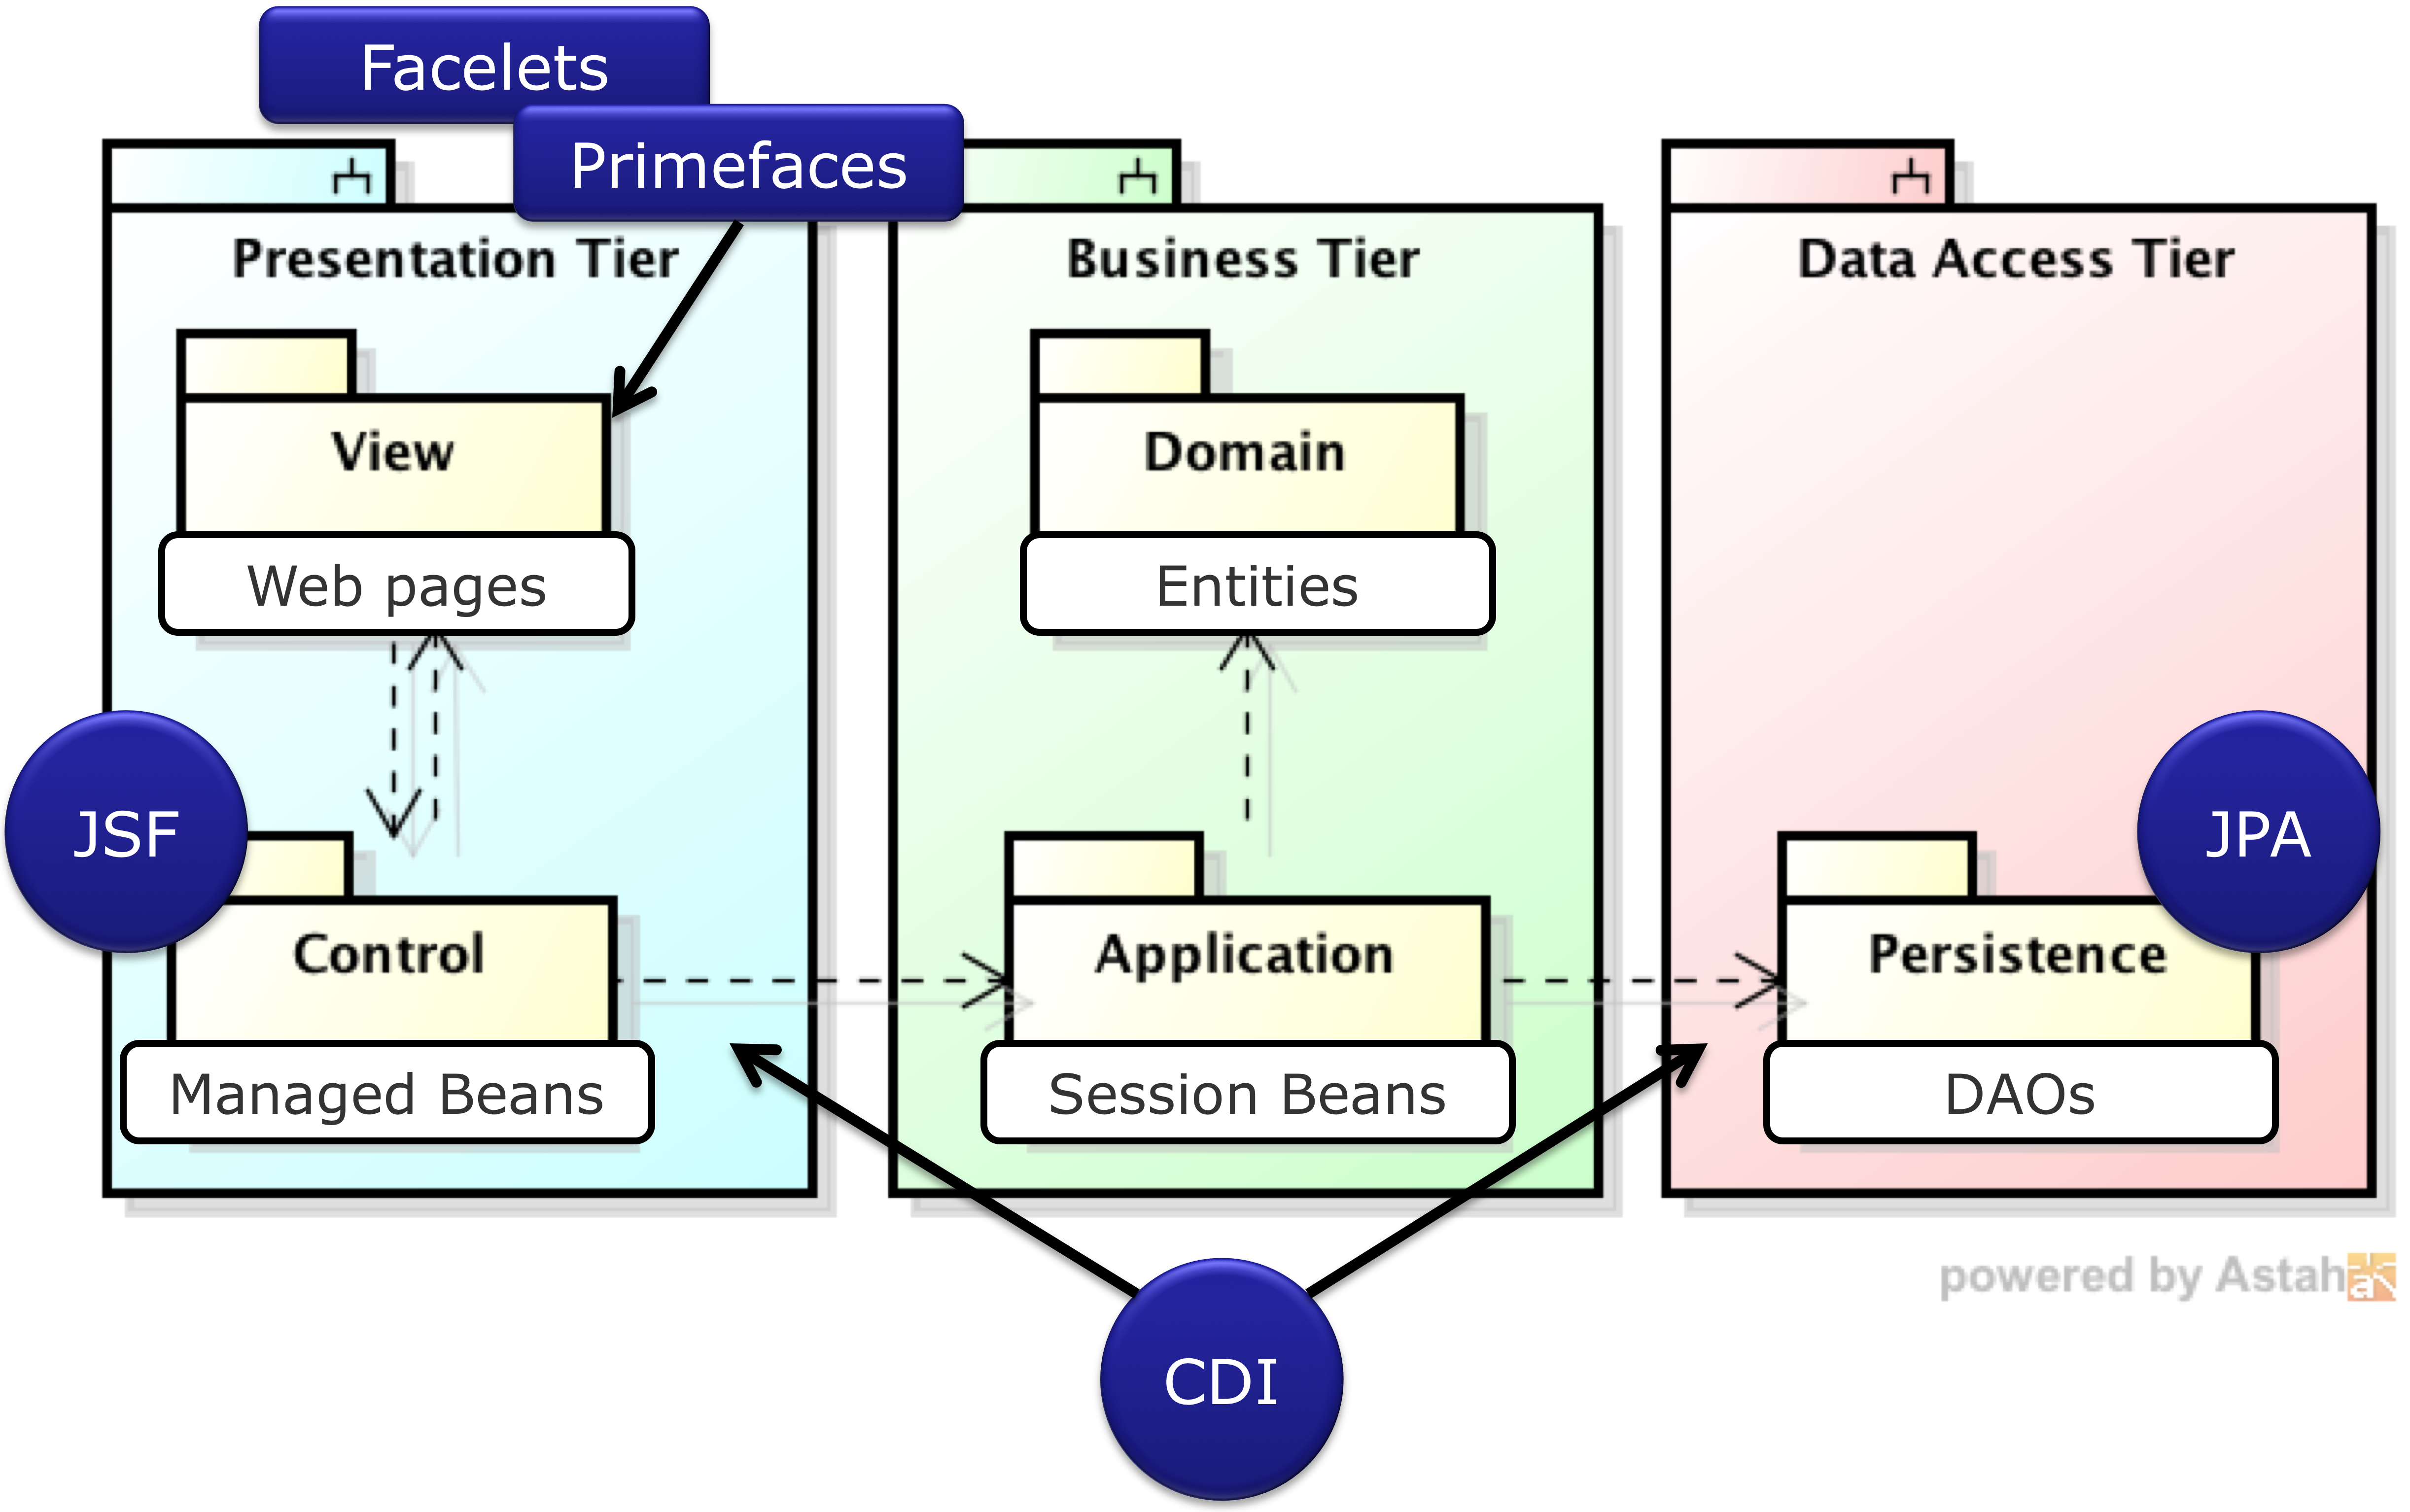
\includegraphics[width=0.8\textwidth]{figuras/figura-arquitetura-padrao.png}
	\caption{Arquitetura de Software.}
	\label{figura-arquitetura}
\end{figure}

\vitor{Substituir a Figura~\ref{figura-arquitetura} pelo diagrama UML da arquitetura do seu projeto e descrevê-la no texto. Caso use alguma arquitetura clássica, incluir referência bibliográfica com BibTeX (ex.:~\cite{fowler:book02}).}

\vspace*{1.5cm}


\chapter{Modelagem FrameWeb}
\label{sec-frameweb}
\vspace{-1cm}

\emph{\imprimirtitulo} é um sistema Web cuja arquitetura utiliza \textit{frameworks} comuns no desenvolvimento para esta plataforma. Desta forma, o sistema pode ser modelado utilizando a abordagem FrameWeb~\cite{souza-celebratingfalbo20}.

A Tabela~\ref{tabela-frameworks} indica os \textit{frameworks} presentes na arquitetura do sistema que se encaixam em cada uma das categorias de \textit{frameworks} que FrameWeb dá suporte. Em seguida, os modelos FrameWeb são apresentados para cada camada da arquitetura.

\vitor{Substituir os valores da segunda coluna da Tabela~\ref{tabela-frameworks} pelos \textit{frameworks} utilizados no seu projeto. Remover o \hl{fundo amarelo}.}


\begin{footnotesize}
	\begin{longtable}{|c|c|}
		\caption{\textit{Frameworks} da arquitetura do sistema separados por categoria.}
		\label{tabela-frameworks}\\\hline
		
		\rowcolor{lightgray}
		\textbf{Categoria de \textit{Framework}} & \textbf{\textit{Framework} Utilizado} \\\hline 
		\endfirsthead
		\hline
		\rowcolor{lightgray}
		\textbf{Categoria de \textit{Framework}} & \textbf{\textit{Framework} Utilizado} \\\hline 
		\endhead

		Controlador Frontal & \hl{JSF} \\\hline

		Injeção de Dependências & \hl{CDI} \\\hline

		Mapeamento Objeto/Relacional & \hl{JPA} \\\hline

		Segurança & \hl{JAAS} \\\hline
	\end{longtable}
\end{footnotesize}




\section{Camada de Negócio}
\label{sec-frameweb-negocio}

\vitor{Apresentar os modelos de entidades e de aplicação do FrameWeb.}




\section{Camada de Acesso a Dados}
\label{sec-frameweb-dados}

\vitor{Apresentar os modelos de persistência do FrameWeb.}



\section{Camada de Apresentação}
\label{sec-frameweb-apresentacao}

\vitor{Apresentar os modelos de navegação do FrameWeb.}


\endgroup



%%% Páginas finais do documento: bibliografia e anexos. %%%
% Finaliza a parte no bookmark do PDF para que se inicie o bookmark na raiz e adiciona espaço de parte no sumário.
\phantompart

% Marca o início dos elementos pós-textuais.
\postextual

% Referências bibliográficas
\bibliography{bibliografia}

% Índice remissivo.
\phantompart
\printindex

% Fim do documento.
\end{document}
